\documentclass[letterpaper,11pt,notitlepage]{article} 
\usepackage[left=2cm,top=2cm,right=2cm,bottom=2cm]{geometry}
% para poder escribir con tildes
\usepackage[T1]{fontenc}
\usepackage[utf8]{inputenc}
\usepackage[spanish]{babel}

% fuentes para escribir símbolos
\usepackage{amsfonts}
\usepackage{amssymb}
\usepackage{amsthm}
\usepackage{mathrsfs}

% inclusión de graficos
\usepackage{graphicx}

% \usepackage{hyperref}
\pagestyle{empty}
\usepackage[centertags]{amsmath}
% Codigo
\usepackage{listings}
% Varias Imagenes en una Figura
\usepackage{subfig}
% //posicion imagen
\usepackage{float}
\usepackage{subfig}
\usepackage[colorlinks=true,urlcolor=blue]{hyperref}
% \topmargin 0 


\usepackage{color}
\definecolor{gray97}{gray}{1}
\definecolor{gray75}{gray}{.75}
\definecolor{gray45}{gray}{.45}
\lstset{ frame=Ltb,
framerule=0pt,
aboveskip=0.5cm,
framextopmargin=3pt,
framexbottommargin=3pt,
framexleftmargin=0.4cm,
framesep=0pt,
rulesep=.4pt,
backgroundcolor=\color{gray97},
rulesepcolor=\color{black},
%
stringstyle=\ttfamily,
showstringspaces = false,
basicstyle=\small\small\ttfamily,
commentstyle=\color{gray45},
keywordstyle=\bfseries,
%
numbers=left,
numbersep=12pt,
numberstyle=\tiny,
numberfirstline = false,
breaklines=true,
}
% minimizar fragmentado de listados
\lstnewenvironment{listing}[1][]
{\lstset{#1}\pagebreak[0]}{\pagebreak[0]}
\lstdefinestyle{consola}
{basicstyle=\scriptsize\bf\ttfamily,
backgroundcolor=\color{gray75},
}
\lstdefinestyle{C}
{language=C,
basicstyle=\ttfamily
}

% ====================================

% % ===== Encabezado =====
% \pagestyle{myheadings}
% \markright{Tutorial Creación de proyecto en MPLABX \hfill }


% ===== Ajuste layout pagina =====
%\usepackage{fullpage}

% ================================

% --- commandos ---
% \newcommand{\ds}{\displaystyle}
% \def\x{{\bf x}}
% -----------------

% ========  Aca comienza el cuerpo del texto ==========
\begin{document}

% \maketitle

\begin{center}
\textsc{ \huge \bfseries Arquitectura de Computadores\\[0.2cm] 543.426}\\[0.2cm]
\textsc{ Ayudante: Antonio Saavedra}\\[0.2cm]
Ayudantía No. 3\\

\today
\end{center}

% \tableofcontents


\subsection*{Problema 1}

\begin{figure}[H]
\begin{center}
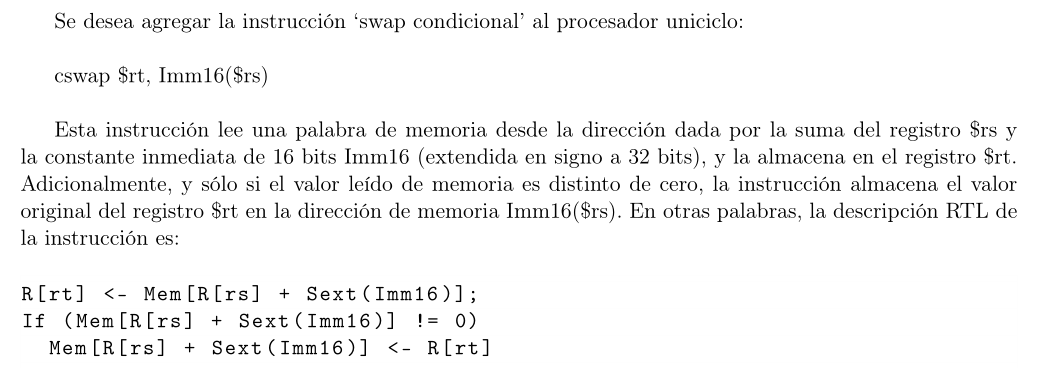
\includegraphics[width=\textwidth]{1.png}
\end{center}
\end{figure}
\begin{figure}[H]
\begin{center}
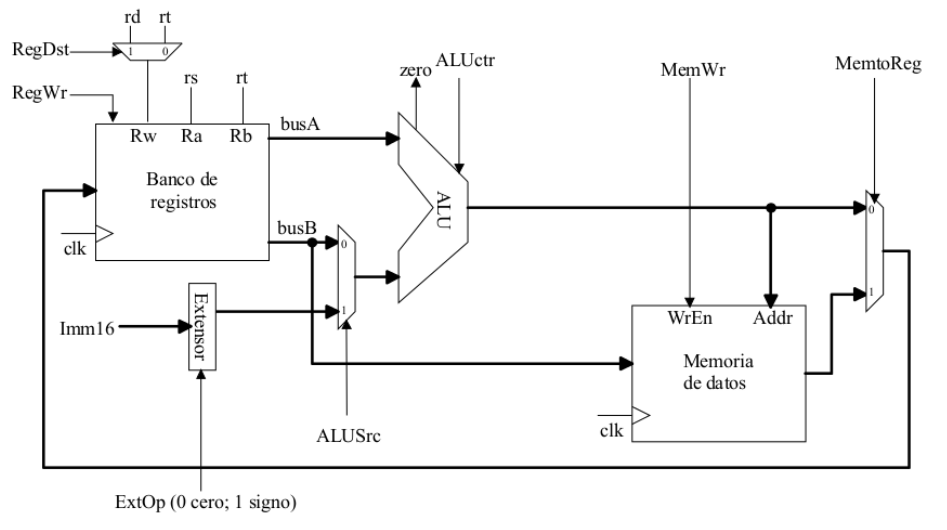
\includegraphics[width=0.88\textwidth,keepaspectratio=true]{unic}
\end{center}
\caption{unicesador Uniciclo}
\end{figure}

\begin{table}[H]
\begin{center}
\begin{tabular}{|c|c|c|c|c|c|c|c|c|} \hline
            & R-type  & ori & andi & lw & sw & beq \\ \hline
RegDst      & 1       & 0   &0     & 0  & x  & x    \\ \hline
ALUSrc      & 0       & 1   &1     & 1  & 1  & 0    \\ \hline
MemtoReg    & 0       & 0   &0     & 1  & x  & x    \\ \hline
RegWr       & 1       & 1   &1     & 1  & 0  & 0    \\ \hline
MemWr       & 0       & 0   &0     & 0  & 1  & 0    \\ \hline
nPC\_sel     & 0       & 0   &0     & 0  & 0  & 1   \\ \hline
ExtOp       & x       & 0   &0     & 1  & 1  & x    \\ \hline
ALUOp       & func    & or  &and   & add& add& sub \\ \hline
  &        &    &    &   &   &    \\ \hline
  &        &    &    &   &   &    \\ \hline
   &        &    &    &   &   &    \\ \hline
\end{tabular}
\end{center}
\end{table}

\newpage
\subsection*{Problema 2}
\begin{figure}[H]
\begin{center}
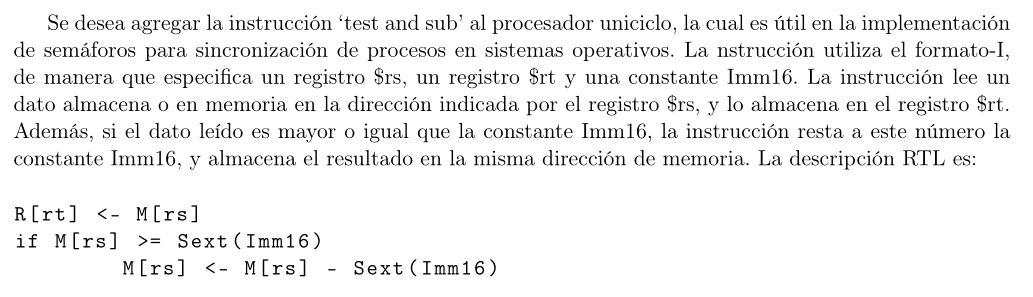
\includegraphics[width=\textwidth]{2.png}
\end{center}
\end{figure}
\begin{figure}[H]
\begin{center}
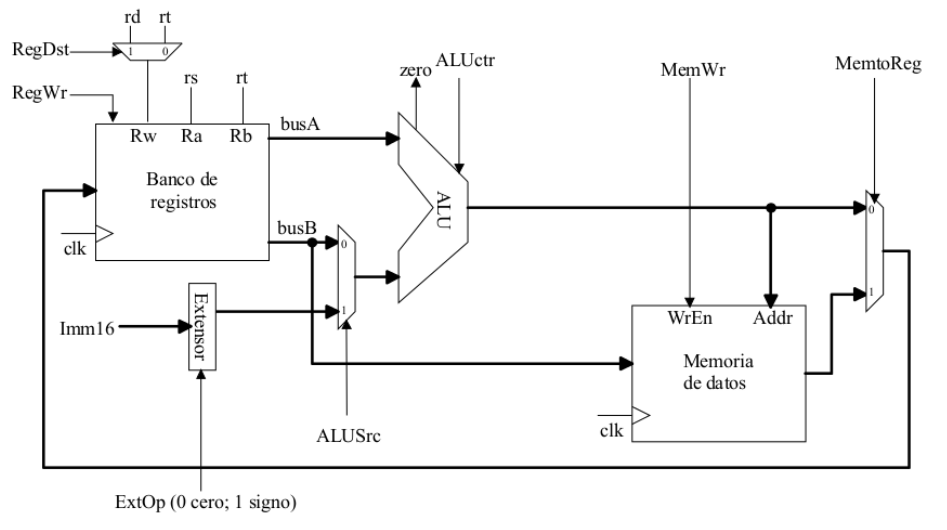
\includegraphics[width=0.88\textwidth,keepaspectratio=true]{unic}
\end{center}
\caption{Procesador Uniciclo}
\end{figure}

\begin{table}[H]
\begin{center}
\begin{tabular}{|c|c|c|c|c|c|c|c|c|} \hline
            & R-type  & ori & andi & lw & sw & beq \\ \hline
RegDst      & 1       & 0   &0     & 0  & x  & x    \\ \hline
ALUSrc      & 0       & 1   &1     & 1  & 1  & 0    \\ \hline
MemtoReg    & 0       & 0   &0     & 1  & x  & x    \\ \hline
RegWr       & 1       & 1   &1     & 1  & 0  & 0    \\ \hline
MemWr       & 0       & 0   &0     & 0  & 1  & 0    \\ \hline
nPC\_sel     & 0       & 0   &0     & 0  & 0  & 1   \\ \hline
ExtOp       & x       & 0   &0     & 1  & 1  & x    \\ \hline
ALUOp       & func    & or  &and   & add& add& sub\\ \hline
  &        &    &    &   &   &    \\ \hline
  &        &    &    &   &   &    \\ \hline
   &        &    &    &   &   &    \\ \hline
\end{tabular}
\end{center}
\end{table}
\subsection*{Problema 3}

\begin{figure}[H]
\begin{center}
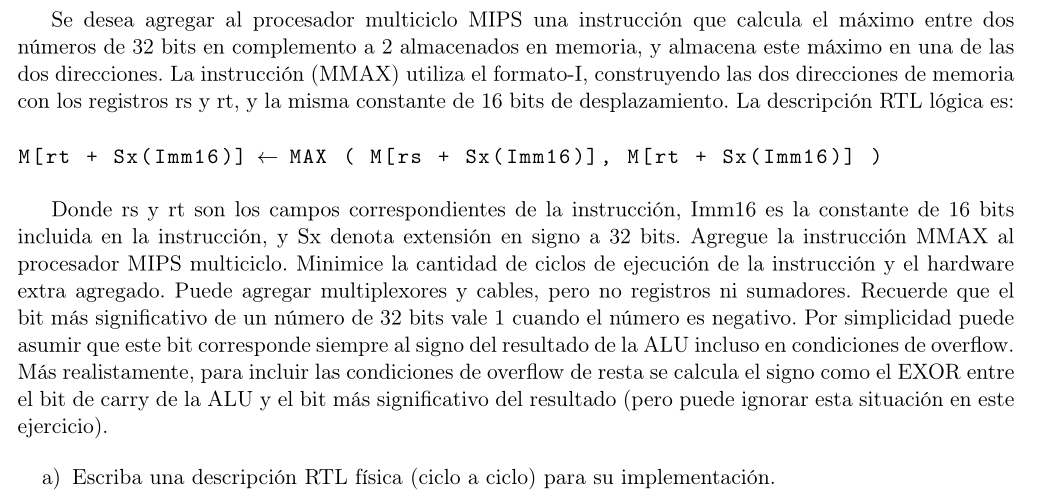
\includegraphics[width=\textwidth]{3.png}
\end{center}
\end{figure}

\begin{figure}[H]
\begin{center}
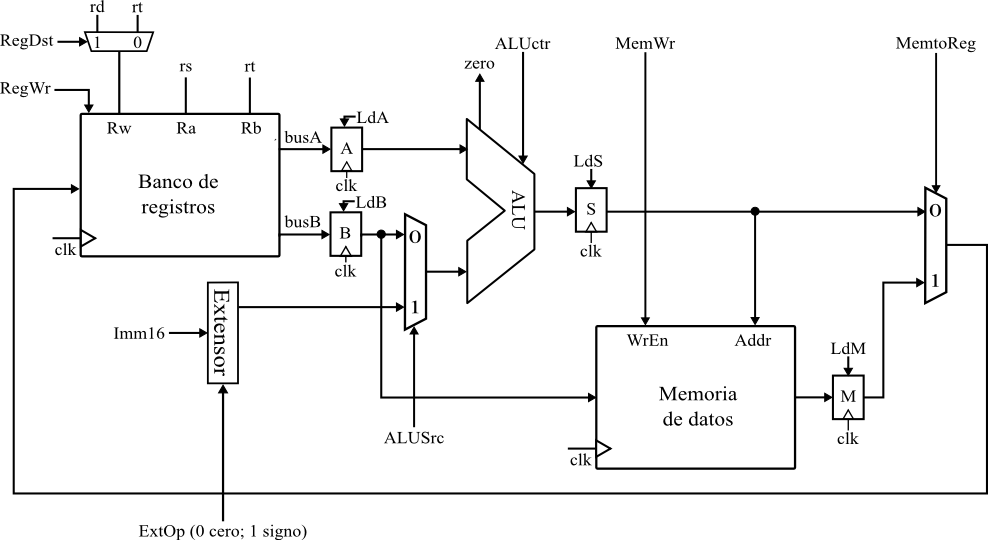
\includegraphics[width=0.88\textwidth,keepaspectratio=true]{proc}
\end{center}
\caption{Procesador Multiciclo}
\end{figure}


\begin{table}[H]
\begin{center}
\begin{tabular}{|c|c|c|c|c|c|c|} \hline
        &(1)&(2)&(3)&(4)&(5) \\ \hline
LdIR    &  &  &  &  &    \\ \hline
RegDst  &  &  &  &  &    \\ \hline
RegWr   &  &  &  &  &    \\ \hline
LdA     &  &  &  &  &    \\ \hline
LdB     &  &  &  &  &    \\ \hline
ExtOp   &  &  &  &  &    \\ \hline
ALUSrc  &  &  &  &  &    \\ \hline
ALUCtr  &  &  &  &  &    \\ \hline
LdS     &  &  &  &  &    \\ \hline
MemWr   &  &  &  &  &    \\ \hline
LdM     &  &  &  &  &    \\ \hline
MemtoReg&  &  &  &  &    \\ \hline
    &  &  &  &  &    \\ \hline
    &  &  &  &  &    \\ \hline

\end{tabular}
\end{center}
\caption{Señales de control por ciclo de instrucción}
\end{table}

\end{document}